\subsection{Automated Reduction}
We noticed that most of the useful feedback terms are actually present in the original query and hypothesized that the baseline system could be substantially improved by removing negative query terms. We used four approaches to refine the initial patent query: 
\begin{enumerate}
  \item removing document frequent terms,
  \item keeping frequent terms in query~\cite{maxwell2013compact},
  \item using pseudo relevance feedback to select query terms, 
  \item removing general terms in IPC title. 
\end{enumerate}

In standard IR, removing terms, appearing a lot in the collection, helps the retrieval effectiveness. Inspired by this fact, we removed the words with average term frequency (in top-100 documents) higher than the threshold $\tau$ from the original query. As it can be seen in figure \ref{fig:queryreduc}, unlike our assumption, removing frequent terms in top-100 documents ($DF(t)>\tau$) ruined the performance.     
\begin{figure}[htpb]
   \centering
   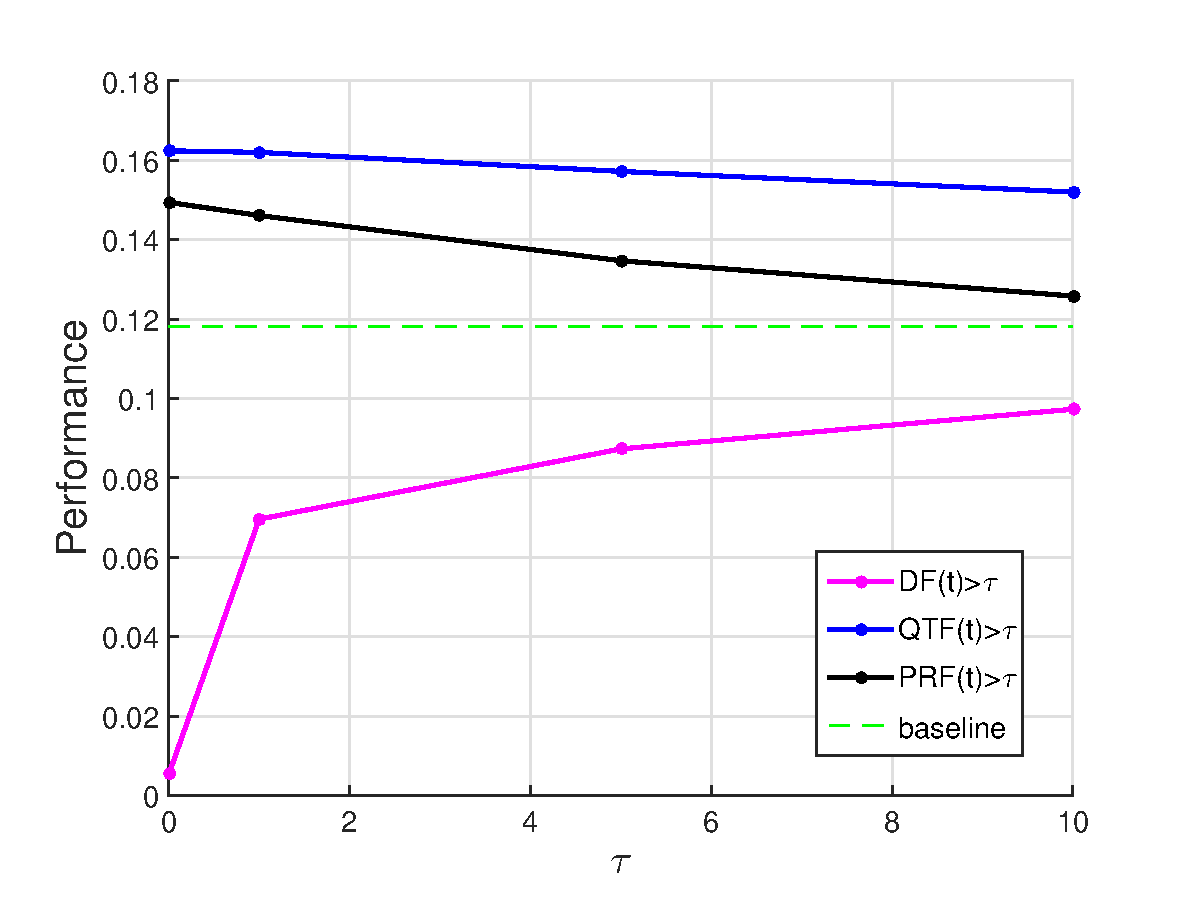
\includegraphics[width=0.30\textwidth,height=40mm]{figs/queryreduc.eps}
   \caption{System performance vs. the threshold $\tau$ for three query reduction approaches.}   
   \label{fig:queryreduc} 
\end{figure}

As mentioned in~\cite{maxwell2013compact} terms inside verbose queries are also important. So, we kept frequent words inside the query while removing document frequent words. It can be seen in Figure \ref{fig:queryreduc} that keeping terms with term frequency higher than a threshold $\tau$ helped and we got the performance when keeping all query terms but it is close to the baseline. 

We used pseudo relevance feedback (PRF) as the third feature to reduce the query. PRF is an automated process without user interaction which assumes the top k ranked documents are relevant and the others are irrelevant. Again, it can be seen in Figure \ref{fig:queryreduc} that the results for query reduction using PRF were below the baseline. In fact, we could not find any heuristic correlates between  $ score_{RF}(t)$ and $ score_{PRF}(t)$. Figure \ref{fig:anecdotal} is an anecdotal example for a sample query which can explain the reason that PRF did not work. It shows the query abstract and a pair of PRF terms, with $ score_{PRF}(t)>10 $, and RF score of each term. It can be seen that terms with high PRF score have a negative RF score which means words from PRF contaminated with sufficient amount of noise to ruin the retrieval effectiveness. 
We used words in IPC code title to reduce the query because as it can be seen in Figure \ref{fig:queryreduc} the majority of them are negative terms as they are general words in all patents belonging to the same category. However we hurt the effectiveness by pruning them out.
\begin{figure}[htpb]
\begin{framed}
\vspace*{-2ex}
  \centering
    %\lstinputlisting[frame=single, basicstyle=\scriptsize\ttfamily , linewidth=\columnwidth,breaklines=true]{code/anecdotale.tex}\vspace*{-2ex}
 \begin{lstlisting}[basicstyle=\tiny\ttfamily , linewidth=\columnwidth,breaklines=true] 
PAC-1612
Abstract: A wireless communication method for transmitting data from at least one master to one or more slaves positioned at various spatial locations and configured for generally simultaneous reception of the data. The method includes dividing the data into a number of portions, transmitting at least some of the portions using different transmission configurations for the different portions, having one or more of the slaves measure the quality of transmission associated with the group of different transmission configurations, and processing the quality measurements to determine new transmission configurations for use in transmitting the data.

PRF Terms: <@\textcolor{red}{commun:-69.43159}@>, <@\textcolor{red}{transmiss:-58.168427}@>, <@\textcolor{red}{wireless:-7.68421}@>, <@\textcolor{red}{telephon:-25.17895}@>, <@\textcolor{red}{recept:-37.810528}@>, <@\textcolor{red}{slave:-31.0421}@>, <@\textcolor{red}{deleg:-22.368422}@>, <@\textcolor{red}{turn:-18.536846}@>, <@\textcolor{red}{master:-35.778954}@>, <@\textcolor{red}{origin:-4.7473674}@>, <@\textcolor{blue}{schedul:12.852628}@>, <@\textcolor{red}{control:-14.842104}@>, <@\textcolor{blue}{frequenc:60.34737}@>, <@\textcolor{red}{station:-76.26316}@>, <@\textcolor{red}{electron:-8.442106}@>, <@\textcolor{red}{perform:-9.71579}@>, <@\textcolor{blue}{band:16.789476}@>, <@\textcolor{red}{termin:-40.04211}@>, <@\textcolor{blue}{indic:3.6210496}@>, <@\textcolor{red}{reason:-6.642107}@>, <@\textcolor{red}{apparatus:-6.2421055}@>, <@\textcolor{red}{determin:-8.97895}@>, <@\textcolor{red}{complet:-8.842103}@>, <@\textcolor{red}{prohibit:-3.8947372}@>, <@\textcolor{red}{state:-9.557897}@>, <@\textcolor{blue}{link:1.1157892}@>, <@\textcolor{blue}{hop:24.378946}@>, <@\textcolor{red}{lan:-8.3368435}@>, <@\textcolor{red}{assign:-9.68421}@>, <@\textcolor{blue}{f1:14.926317}@>, <@\textcolor{red}{short:-3.6000004}@>, <@\textcolor{blue}{pattern:17.58947}@>, <@\textcolor{blue}{paramet:1.5473672}@>, <@\textcolor{red}{serv:-4.5684214}@>, <@\textcolor{blue}{permit:0.62105286}@>

IPC def Terms: <@\textcolor{red}{network: -28.557888}@>, <@\textcolor{red}{traffic: -3.2526314}@>, <@\textcolor{red}{resourc: -1.2947367}@>, <@\textcolor{red}{manag: -9.652633}@>, <@\textcolor{red}{local: -6.1368427}@>, <@\textcolor{red}{wireless: -7.68421}@>, <@\textcolor{blue}{schedul: 12.852628}@>, <@\textcolor{blue}{select: 13.473684}@>, <@\textcolor{red}{alloc: -10.042107}@>, <@\textcolor{red}{switch: -14.463159}@>, <@\textcolor{red}{interconnect: -0.5578947}@>, <@\textcolor{red}{transfer: -4.5052633}@>, <@\textcolor{red}{inform: -43.400013}@>, <@\textcolor{red}{signal: -30.71579}@>, <@\textcolor{red}{memori: -9.094736}@>, <@\textcolor{red}{input: -9.736838}@>, <@\textcolor{red}{plan: -0.22105263}@>, <@\textcolor{red}{coverag: -0.4526316}@>, <@\textcolor{red}{tool: -0.15789473}@>, <@\textcolor{red}{deploy: -0.07368421}@>, <@\textcolor{red}{partit: 0.0526316}@>, <@\textcolor{red}{cell: -7.6842103}@>, <@\textcolor{red}{structur: -0.94736844}@>, <@\textcolor{red}{orthogon: -4.1789474}@>, <@\textcolor{red}{multiplex: -11.621052}@>, <@\textcolor{red}{walsh: -0.29473686}@>, <@\textcolor{red}{code: -27.842102}@>, <@\textcolor{red}{supervisori: -0.16842104}@>, <@\textcolor{red}{monitor: -6.7157907}@>, <@\textcolor{red}{test: -1.2210523}@>, <@\textcolor{red}{arrang: -0.5578947}@>, <@\textcolor{red}{spread: -2.7263162}@>, <@\textcolor{red}{spectrum: 3.6000001}@>, <@\textcolor{red}{direct: -1.810526}@>, <@\textcolor{red}{sequenc: -3.9052625}@>, <@\textcolor{red}{modul: -16.0}@>, <@\textcolor{blue}{frequenc: 60.34737}@>, <@\textcolor{blue}{hop: 24.378946}@>, <@\textcolor{red}{radio: -15.242106}@>, <@\textcolor{red}{transmiss: -58.168427}@>, <@\textcolor{red}{radiat: -0.3157895}@>,  <@\textcolor{red}{mobil: -6.831579}@>, <@\textcolor{red}{mainten: -0.75789464}@>, <@\textcolor{red}{administr: -0.07368421}@>, <@\textcolor{red}{path: -1.6631576}@>, <@\textcolor{red}{configur: -9.094739}@>, <@\textcolor{red}{lan: -8.3368435}@>, <@\textcolor{blue}{wide: 0.021052642}@>, <@\textcolor{red}{wan: -0.021052632}@>
 \end{lstlisting} 
 \vspace*{-2ex}
\end{framed}
 \vspace*{-2ex}
  \caption{Anecdotal example: it shows the abstract, and $ term: \; score_{RF}(term) $ pair of a sample query. Useful terms are highlighted in blue and the noisy ones in red.}
  \label{fig:anecdotal}  
\end{figure}
%\vspace*{-2ex}

Unlike our initial assumption, non of the standard proposed query reduction approaches for query reduction worked better than the baseline.
\subsection{Reduction by Relevance Feedback}
All our attempts to improve the system effectiveness without accessing the relevance feedback were quite in vein because the features we recognized were tightly the combination of the useful words and noisy words and the system performance is too sensitive to the existence of a noisy word or the absence of the useful terms. So, we decided to apply much more realistic approach in which feedback terms are extracted only from the first ranked relevant document retrieved. Table \ref{tab:firstrel} shows that we can double the MAP by only the first-ranked relevant document.
\begin{table}[htpb]
  \begin{center}
   \caption{System performance using minimal relevance feedback. $\tau$ is RF score threshold, and $k$ indicates the number of first relevant retrieved patents.}\vspace{3mm}
  \input table/partialRFtermselect.tex   
  \label{tab:firstrel}
  \end{center}  
\end{table}
Fig. \ref{fig:FirstTPRankHisto} indicates that the baseline methods return a relevant patent, approximately, 80\% of the time in the first 10 results and 90\% of the time in the first 20 results, such an interactive approach requires relatively low user effort while achieving state-of-the-art performance.    
\begin{figure}[htpb]
   \centering
   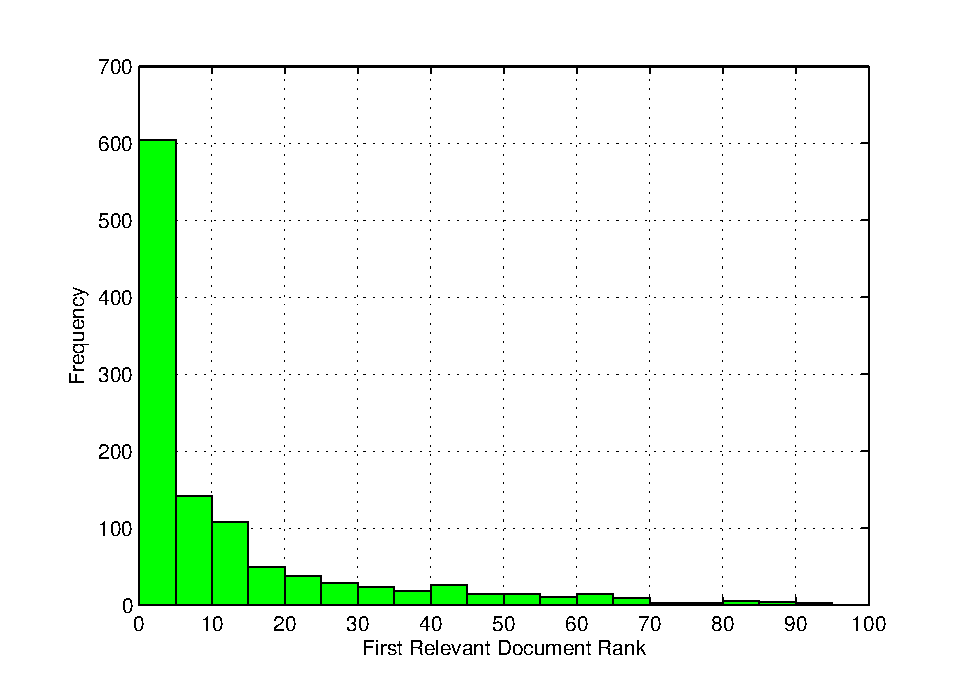
\includegraphics[width=0.25\textwidth,height=32mm]{figs/FirstTPRank.eps}
   \caption{The distribution of the first relevant document rank over test queries which have TPs}   
   \label{fig:FirstTPRankHisto} 
\end{figure}